\chapter{Results and Discussion}
\label{Ch:Result and Discussion}
\section{Q-Learning}

\subsection{Basic Model}
To build basic model, we used portfolio value change as a reward function, which means the agent will choose the action that will increase the expected portfolio value the most. We used two decimal of price change pair as a state.

We adjusted the parameters to give better performance. The learning rate($\alpha$), which decides the impact of new data on the existing Q-table, was set as 0.0001 based on experiment. The discount factor($\gamma$), which discounts the sum of future reward was set as 0.9. The epsilon($\epsilon$) was set as 0.9 and for every time period it is decreased 1\% until it reaches 0.01. It is in order to let the actions be chosen more randomly for exploration in the earlier times, since Q-table doesn’t contain much information. However later times’ actions are more likely to be chosen based on Q-table with smaller epsilon value. With those parameters, we trained the Q-table for each dataset 3000 episodes each.

As we trained on 10 training datasets, the performances of the basic model on each dataset didn’t have distinct patterns. Usually, the portfolio gains by the model were way better(3~4 times final portfolio value) than benchmark, but training results from 4th, 7th, 8th, 9th training set were similar or even below the benchmark gains. Each plot below has two subplots. The upper plot shows how the final portfolio value changes over every episode, and using the last episode’s data we drew bottom plot which shows the portfolio value change over days. Compared to those of training 1 with KLAC and SKX data and training 10 with NVDA and SKX data, the results of training 4 and training 9 are not good. We didn’t find any clear reason behind this. The dimension of Q-table is steadily increased with more training as shown in below plot.

\begin{figure}[H]
\begin{subfigure}{.5\textwidth}%
\centering
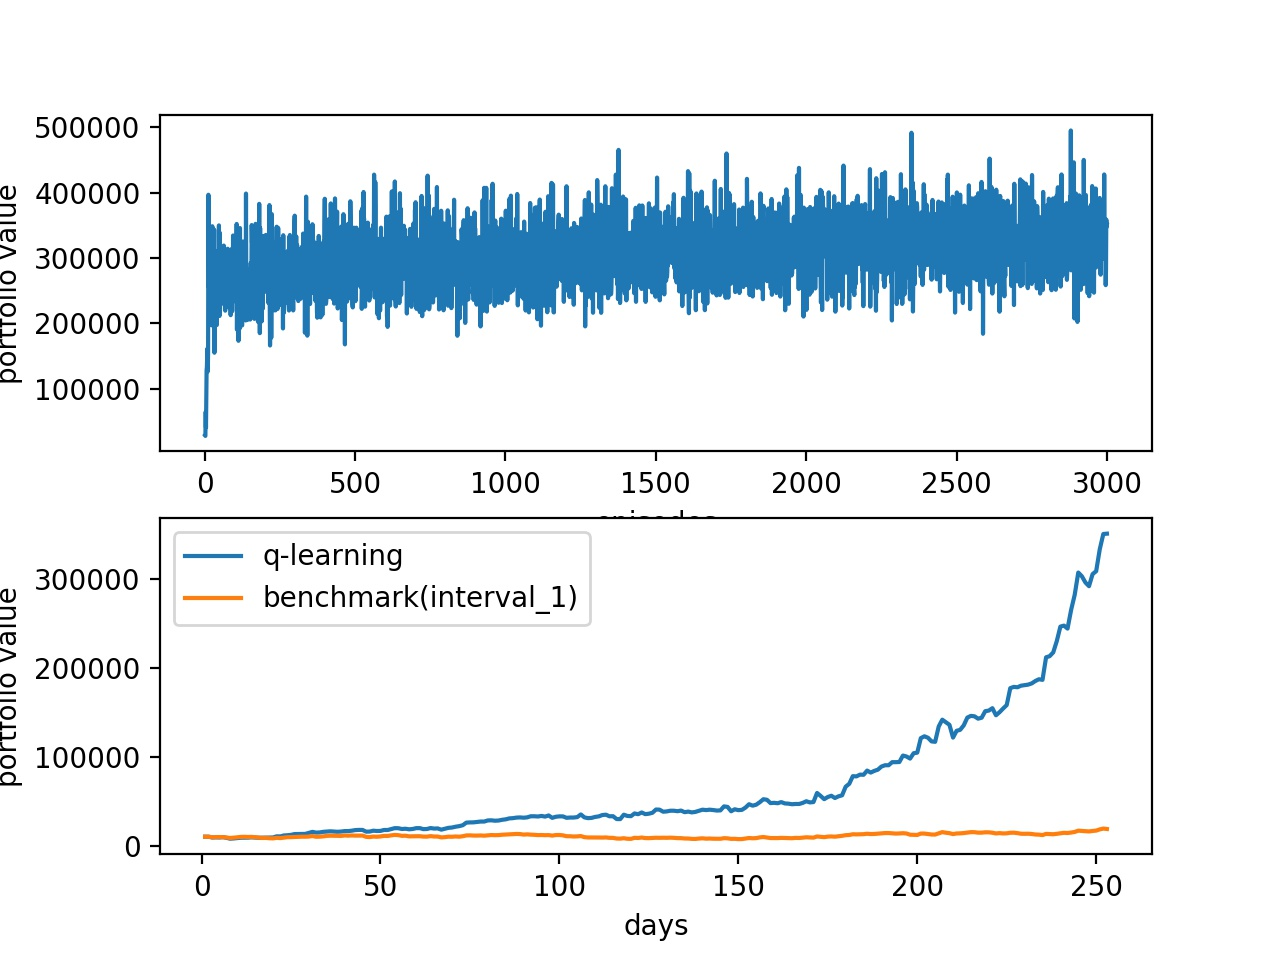
\includegraphics[clip, width=1.1\textwidth]{Graphics/q_learning_KS1.eps} \caption{Training 1 (KLAC \& SKX)} 
\end{subfigure}%
\begin{subfigure}{.5\textwidth}%
\centering
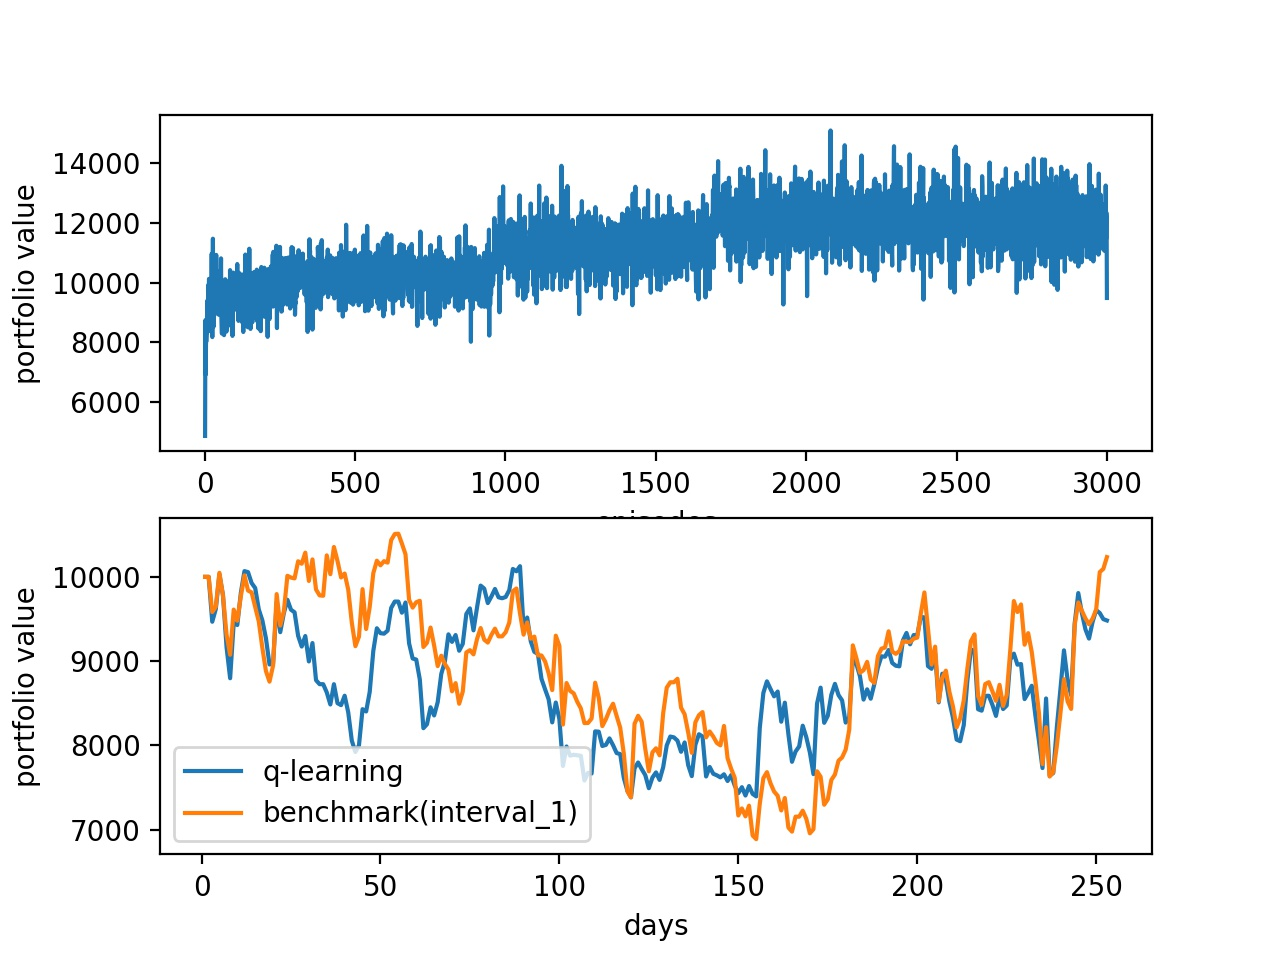
\includegraphics[clip, width=1.1\textwidth]{Graphics/q_learning_AM4.jpg} \caption{Training 4 (AMD \& MTN)}
\end{subfigure}%
\vspace{0.1cm}
\begin{subfigure}{.5\textwidth}%
\centering
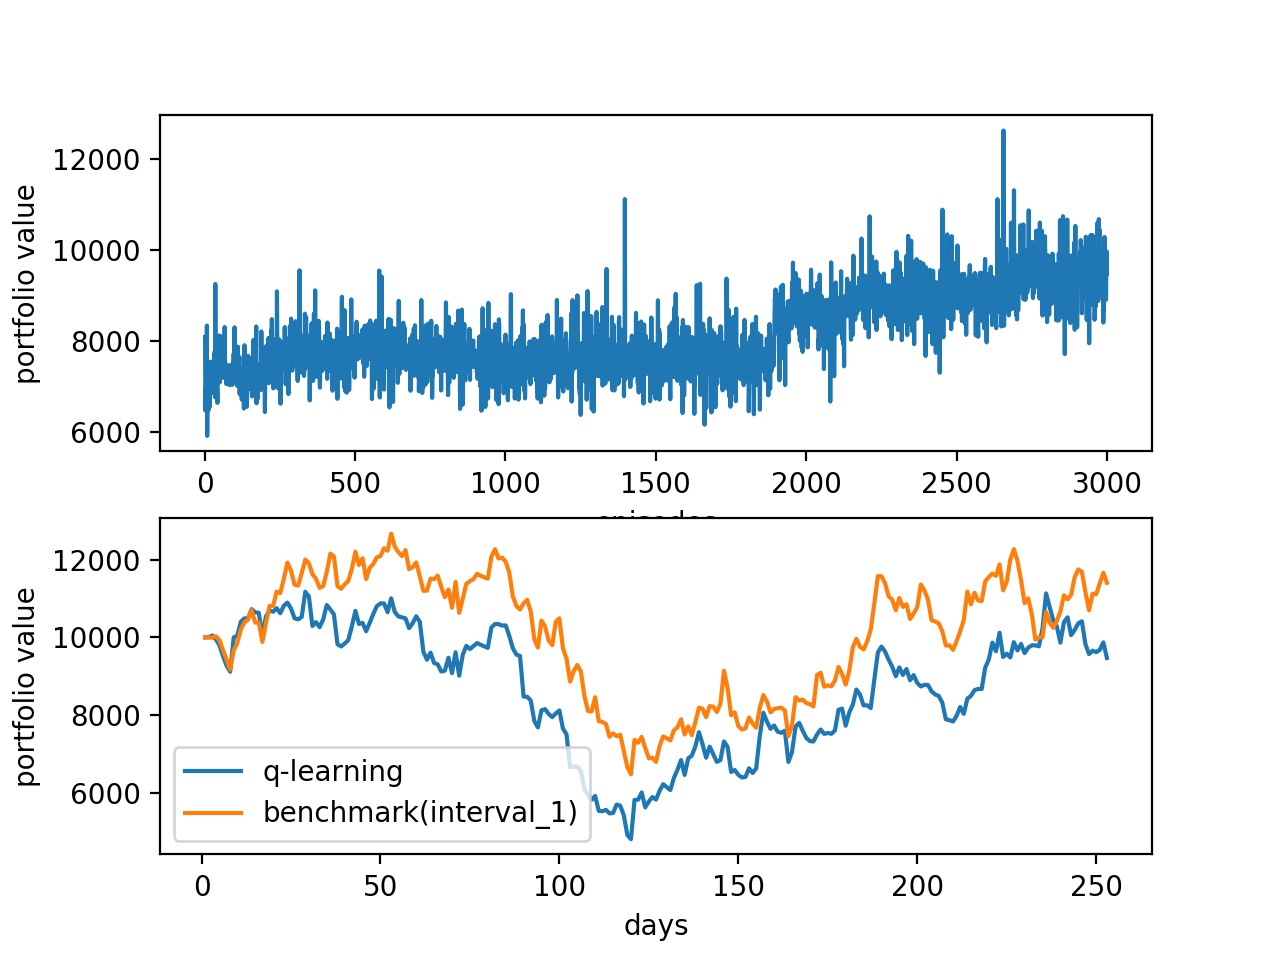
\includegraphics[clip, width=1.1\textwidth]{Graphics/q_learning_MP9.jpg} \caption{Training 9 (MU \& PPC)}
\end{subfigure}%
\begin{subfigure}{.5\textwidth}
\centering
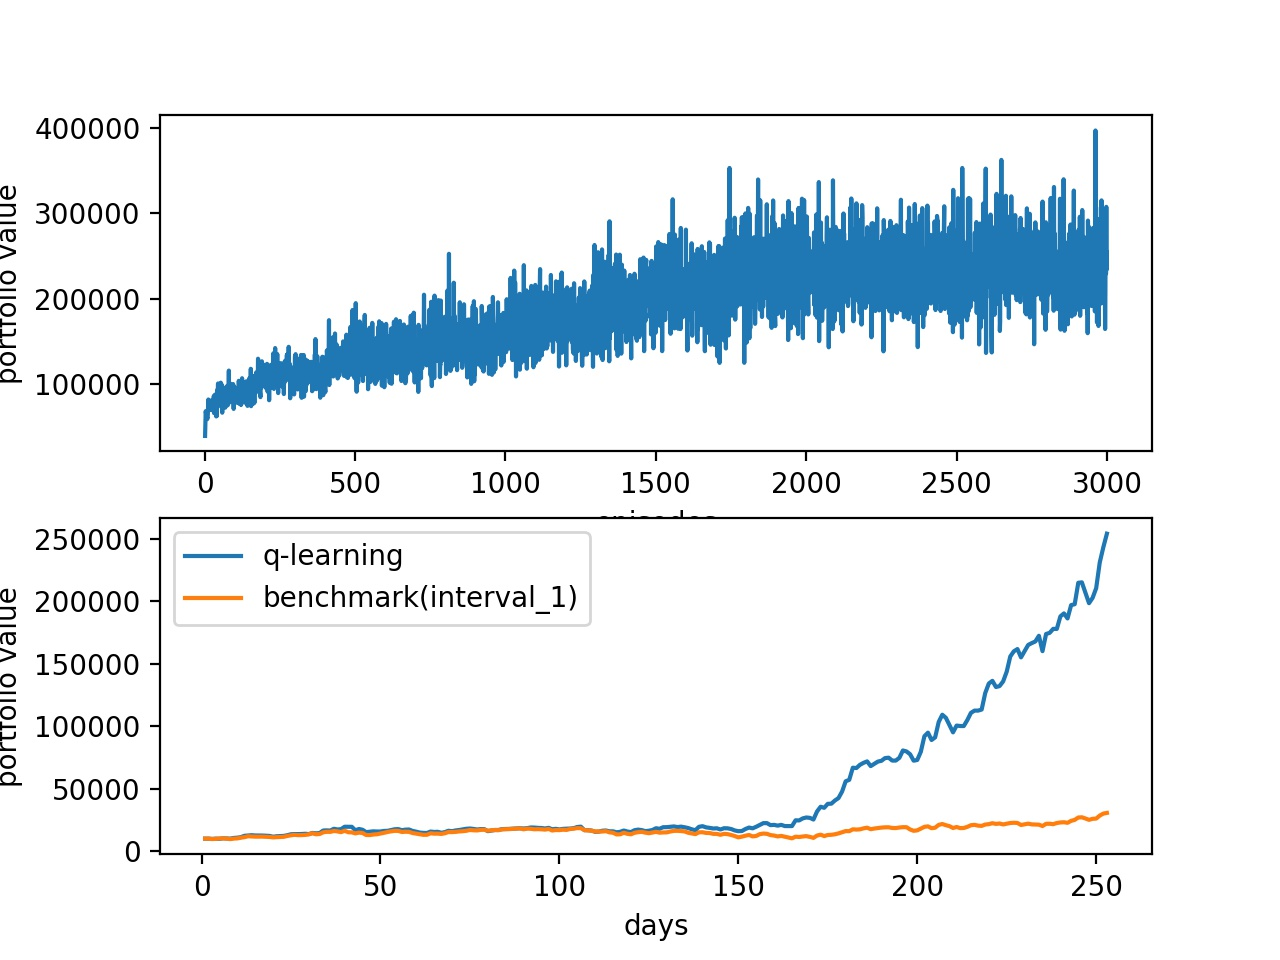
\includegraphics[clip, width=1.1\textwidth]{Graphics/q_learning_NS10.jpg} \caption{Training 10 (NVDA \& SKX)}
\end{subfigure}%
\vspace{0.1cm}
\begin{figure}
\begin{center}
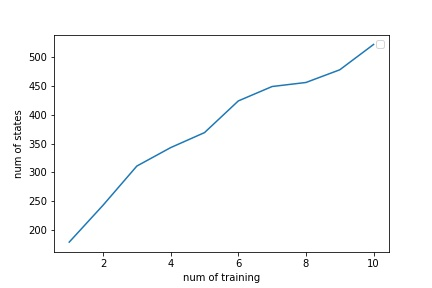
\includegraphics[clip, width=0.8\textwidth]{Graphics/dimension.jpg} \caption{Dimension change over training}
\end{center}
\end{figure}
\end{figure}%

Using the $Q$-table we trained, we tested on two test datasets(AMAT \& CAJ, FCX \& CAJ). Test results using FCX \& CAJ dataset usually showed better results. However more training didn’t guarantee better test results. For AMAT \& CAJ, the best test result was using the Q-table trained with 1 dataset, and further training tables made the test results’ portfolio value be decreased. On the other hand, for FCX \& CAJ, the best test result was with 8 times training Q-table, and before and after that the final portfolio value is below benchmarks. To check the reason why test results keep changing, we analyzed the actions taken in each result. Even the actions taken in the test using 9 times training, and using 10 times training differed a lot. The last plot which has 3 subplots is drawn using the FCX \& CAJ data. The first subplot is comparing the actions taken with 5 and 8 times training, while the second is comparing 8 times and 10 times, and the last is comparing 10 times and 9 times.
\vspace{0.05cm}
\begin{figure}[H]
\begin{center}
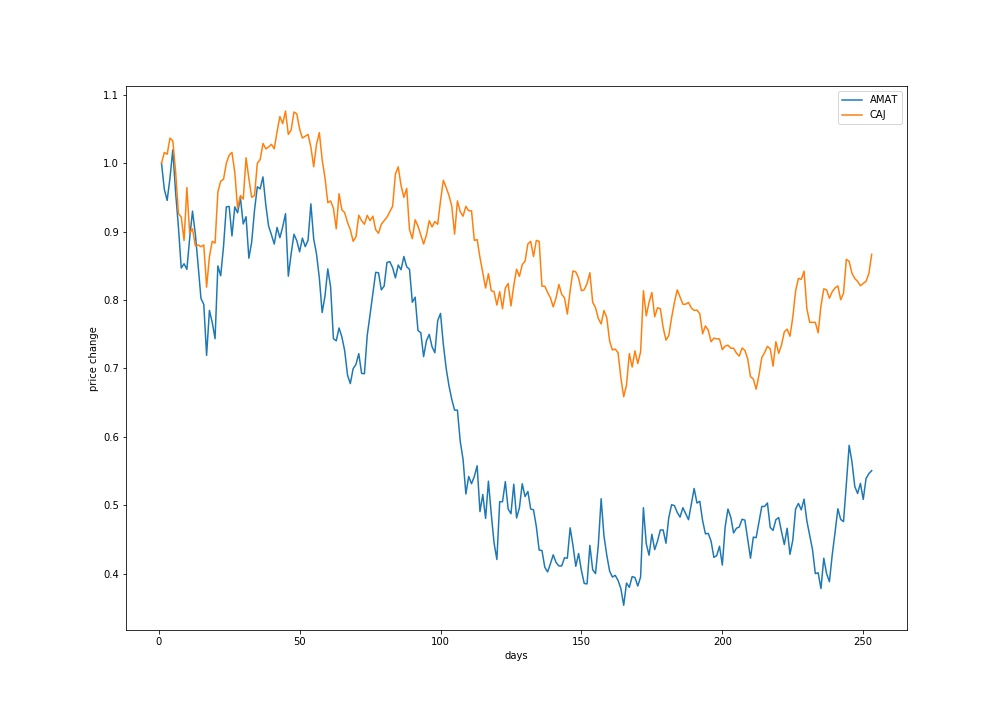
\includegraphics[clip, width=0.8\textwidth]{Graphics/test1_pricechange.jpg} \caption{TEST SET1 (AMAT \& CAJ) :PRICE CHANGE}
\end{center}
\end{figure}

\newpage

\begin{figure}[H]
\begin{subfigure}{.5\textwidth}%
\centering
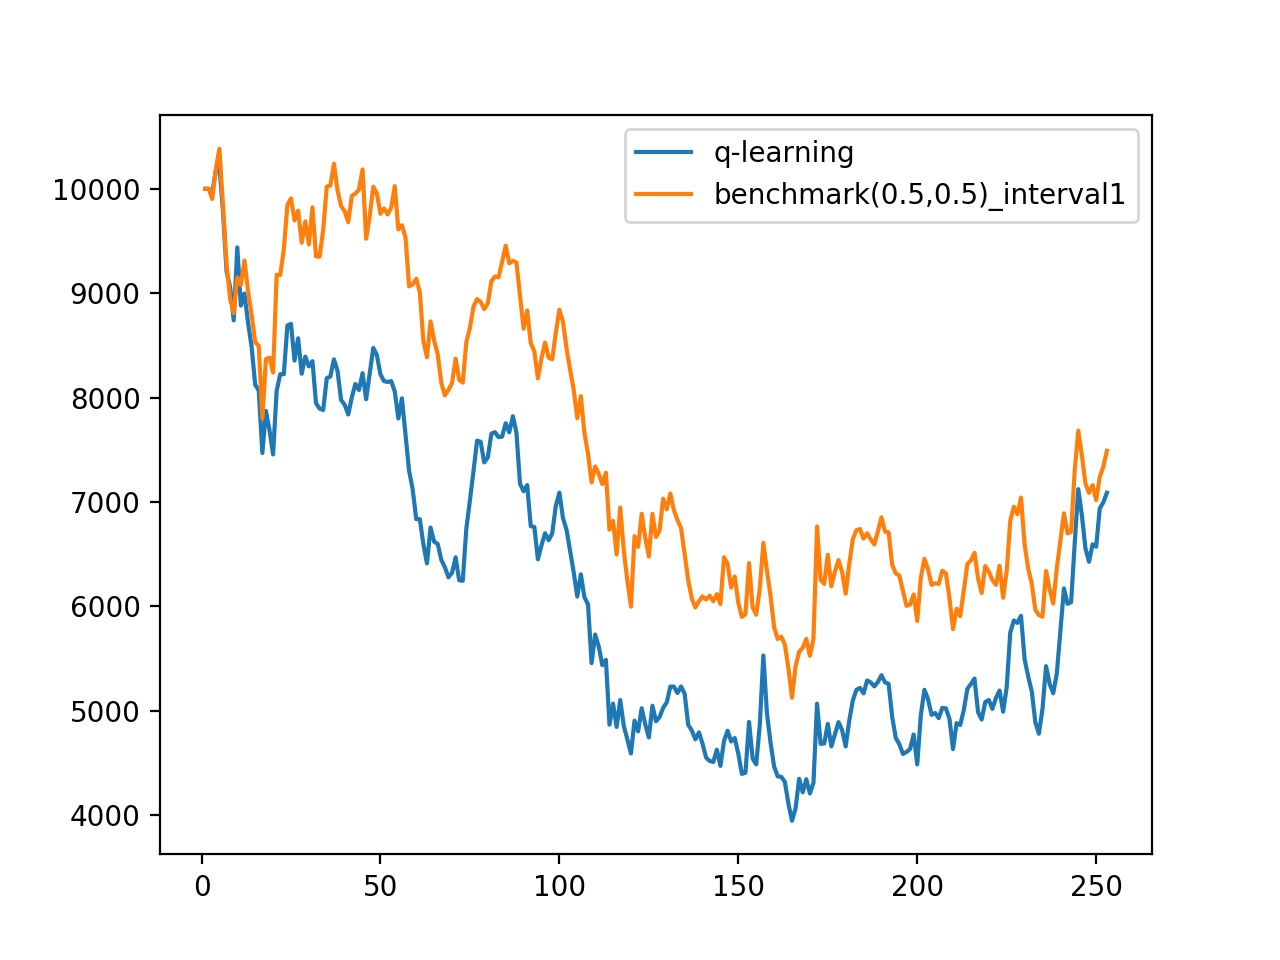
\includegraphics[clip, width=1.1\textwidth]{Graphics/test_KS1_AC_action.jpg} \caption{TEST SET1 (AMAT \& CAJ):1 training} 
\end{subfigure}%
\begin{subfigure}{.5\textwidth}%
\centering
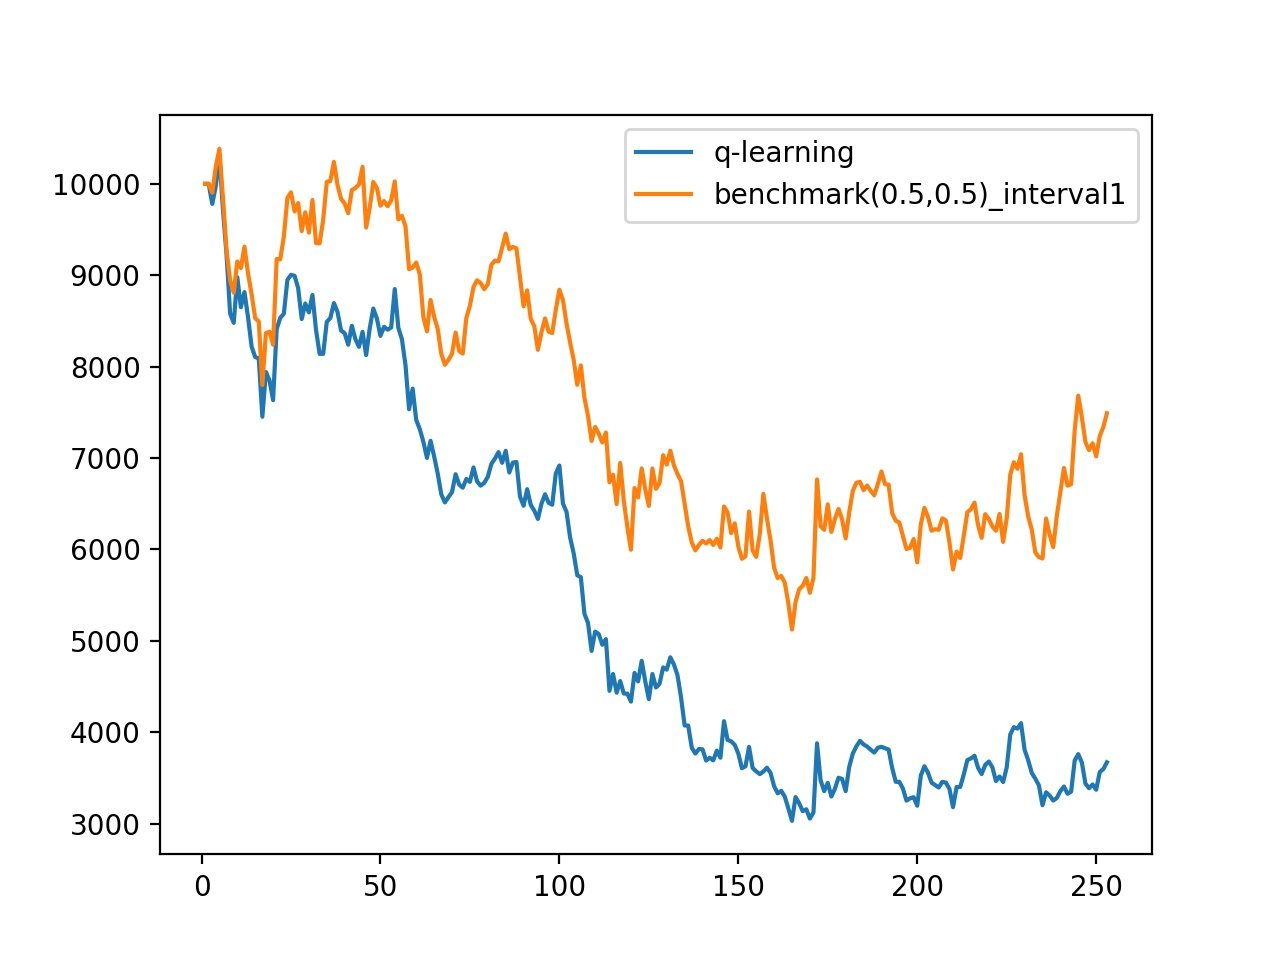
\includegraphics[clip, width=1.1\textwidth]{Graphics/test_LP3_AC_action.jpg} \caption{TEST SET1 (AMAT \& CAJ):3 training}
\end{subfigure}%
\end{figure}%

\subsection{Linear Regression}

\section{Deep Q-Network}

Q-learning has some obvious problems in our problem setting.
Firstly, to implement Q-learning we have to discretize the state, which is the stock price. However, if we discretize the stock price, the result we get will be inaccurate, which implies that the profit we get may not be optimized. Thus, it is necessary to find an alternative way that can handle the continuous state situation.

Secondly, the action state can also be continuous . It is impossible to find all the Q-value corresponding to each actions for a state. Computer should be able to find action that fits our goal the most even when it runs into entirely new situation, but if Q-table values that computer finds are not enough computer will choose the action randomly. Thus, it is necessary to find another way that helps the computer find the right action without having to find out every single Q-table value directly.

To solve these two big problems, Deep Q Network is an appropriate method to solve them.

In our Deep Q Network algorithm, computer chooses action randomly with pre-determined probability, which is called ‘epsilon exploration’. It is mainly used in stochastic process like this situation where stock price changes randomly, because if without this epsilon exploration after one certain state happens computer choose the action depending on this specific state solely even though there are high probabilities the other states can happen as well. 
When neural networks are trained, we use mini-batch which picks items randomly in the memories which consists of plenty of pairs of state, action, reward, and next-state. In Q-learning, Q-table is updated with time and it is affected by time correlation. Unlike Q-learning, in Deep Q Network this algorithm called ‘Experience Replay’ is used to avoid correlation between each memory, especially with this kind of situation where time is related with, and it makes results better.     

In this project, fully connected layers, whose inputs are vectors, are used instead of convolutional neural networks, whose inputs are matrixes, because states in this project are price changes, which can be expressed more easily as vectors than matrixes. 

Relu and linear function are used as an activation function, Mean Squared Error function as a loss function, and Adam function as an optimizer. In terms of hyperparameters, we chose figures similar to those that are mainly used. 

\subsection{Including Exchange Ratio}
In the later state of the project, we try to include the exchange ratio into our consideration. The application is that you can include two different countries' stock into the portfolio and settle at the end of the date with one of the stocks' currency in the portfolio. Since sometime due to the difference of public holiday and time-zone in different countries, we may face the situation that one country's stock market is working while the other one is not. When we face such situation, we will just skip that date in our training model.

The way we calculate the portfolio value is as follows
$$ pv_{t} = pv_{t-1} *[ (p_{t} / p_{t-1}) * w_{1}  + (q_{t} / q_{t-1}) * w_{2} * cv_{t}/cv_{t-1})]$$
the portfolio value will be in the currency you have chosen.
\endinput


